\begin{frame}
\end{frame}

\begin{frame}
  \frametitle{授课教材}
  \begin{figure}
    \centering
    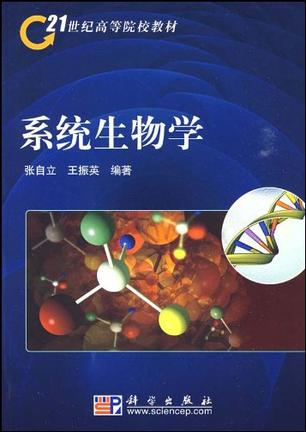
\includegraphics[width=5cm]{c0.book.jpg}
  \end{figure}
\end{frame}

\begin{frame}
  \frametitle{课程安排 | 理论课}
  \begin{table}
    \centering
    \rowcolors[]{1}{blue!20}{blue!10}
    \begin{tabular}{clcc}
      \hline
      \rowcolor{blue!50}顺序 & 授课内容 & 学时 & 授课教师\\
      \hline
      1 & 概论 & 2 & 伊现富\\
      2 & 基因组学 & 6 & 伊现富\\
      3 & 转录组学 & 6 & 伊现富\\
      4 & 蛋白质组学实验技术 & 6 & 王景玉\\
      5 & 糖/代谢物/互作/表型组学 & 10 & 王举\\
      6 & 建模和仿真 & 6 & 王举\\
      7 & 分子进化与系统发育分析 & 2 & 王举\\
      8 & 大作业 & 10 & 张涛\\
      9 & 课堂讨论 & 4 & 王、张、伊\\
      10 & 课程复习 & 2 & 王、王、伊\\
      \hline
    \end{tabular}
  \end{table}
\end{frame}

\begin{frame}
  \frametitle{课程安排 | 实验课}
  \begin{table}
    \centering
    \rowcolors[]{1}{blue!20}{blue!10}
    \begin{tabular}{cllcc}
      \hline
      \rowcolor{blue!50}顺序 & 实验内容 & 理论知识 & 学时 & 授课教师\\
      1 & 测序数据质控与预处理 & 基因组 & 3 & 伊现富\\
      2 & 外显子组测序数据分析 & 基因组 & 3 & 伊现富\\
      3 & 转录组测序数据分析 & 转录组 & 3 & 伊现富\\
      4 & 质谱联用数据分析& 蛋白质组学 & 3 & 王举\\
      5 & 生物系统的建模与仿真& 建模与仿真 & 3 & 王举\\
      6 & 分子进化及系统发育分析& 进化与系统发育 & 3 & 王举\\
      \hline
    \end{tabular}
  \end{table}
\end{frame}

% \begin{frame}
%   \frametitle{考核方式}
%   \begin{enumerate}
%     \item 理论课:50\%
%       \begin{enumerate}
%         \item 平时表现:10\%
%         \item 闭卷考试:40\%
%       \end{enumerate}
%     \item 实验课:30\%
%       \begin{enumerate}
%         \item 平时表现:10\%
%         \item 实验报告:20\%
%       \end{enumerate}
%     \item 课堂讨论:20\%
%       \begin{enumerate}
%         \item 报告答辩:10\%
%         \item 报告论文:10\%
%       \end{enumerate}
%   \end{enumerate}
% \end{frame}

